\chapter{Implementation}
\section{Software architecture}
Continue the IMP tool, all the functions for this task was saved in the \textbf{impls\_2015} package of program. Besides the method was created by myself, I also use some methods from the OpenCV (library for image processing) and Qt framework (framework for C++).\\[0.2cm]
\begin{figure}[h!]
\centering
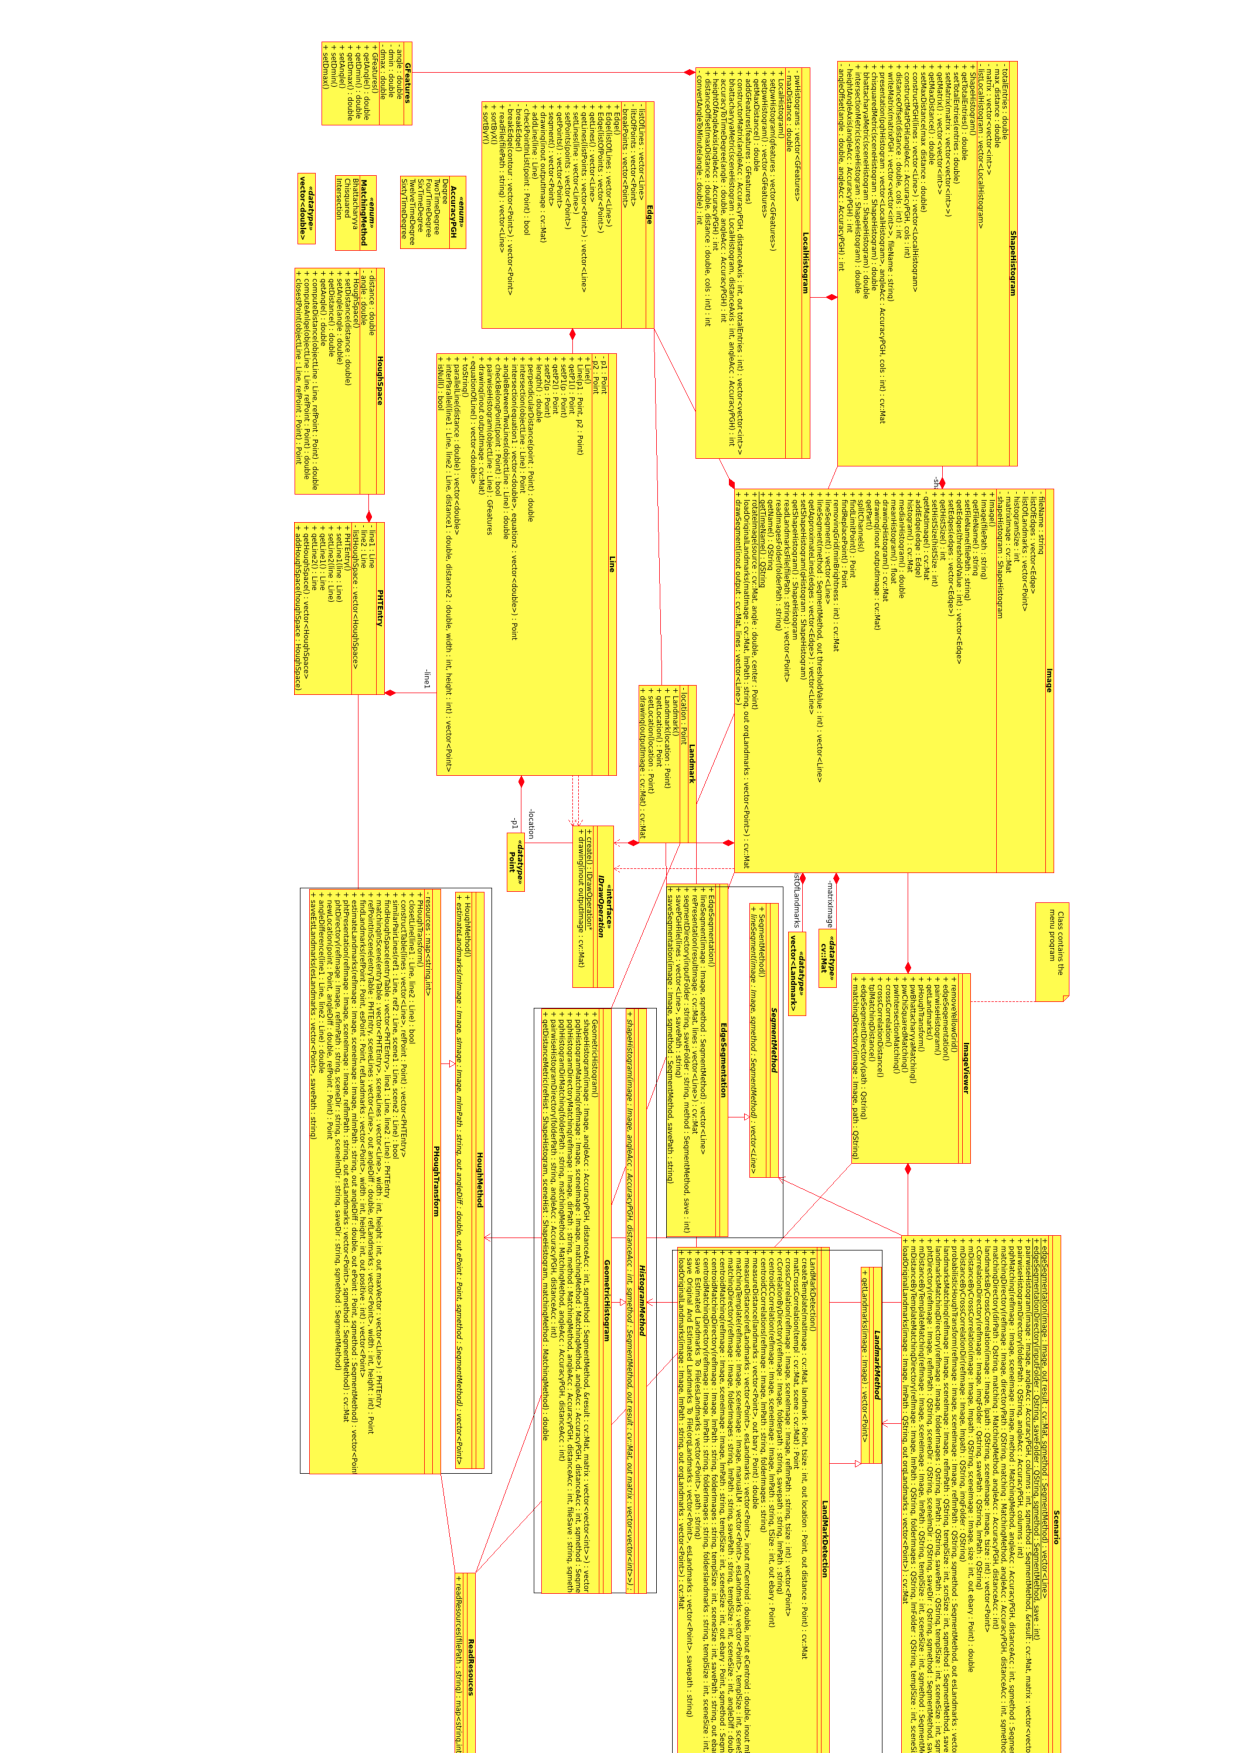
\includegraphics[width=0.9\textwidth]{images/cdiagram}
\caption{The class diagram of program}
\label{fig:cdiagram}
\end{figure}
The class diagram\footnote{See the full image in Appendix} in \ref{fig:cdiagram} show mainly classes of my task. The \textit{mainly} methods located in the \textit{ImageViewer} class, where contains all functions of the software. To represent the information of image and preprocessing about clear the yellow grid, we use the classes such as \textit{Line}, \textit{Edge}, \textit{Landmark}, \textit{YellowGird}, \textit{Image} class. For the edge segmentation, construct the pairwise geometric histogram, probabilistic hough transform and landmarks detection, we have \textit{GFeatures}, \textit{LocalHistogram}, \textit{ShapeHistogram}, \textit{EdgeSegmentation}, \textit{PHTransform} \textit{LandmarkDection} class. The main functions were inherated from the abstract classes \textit{HistogramMethod}, \textit{SegmentMethod}, \textit{HoughMethod}, \textit{LandmarkMethod} respective and used in \textit{main} class (\textit{ImageViewer}) via the \textit{Sceneario} class. The description, properties and methods in each class was discussed in below sections.
\section{Image preprocessing}
The \textit{Image processing} section describes the information about the classes which describe the geometric objects can be represent the image and the method to remove the yellow grid on the images.
\subsection{Line class}
\textbf{Line} class describe the information of a straight line and the methods can do with a line.
\subsubsection{The attributes}
\begin{itemize}
\item\textbf{p1}: the first endpoint of line.
\item\textbf{p2}: the second endpoint of line.
\end{itemize}
\subsubsection{The methods}
\begin{itemize}
\item\textbf{Line()}: Constructor an empty line.
\item\textbf{Line(p1: Point, p2: Point)}: Constructor a line with two endpoints p1, p2. With type of the endpoints is \textbf{Point} (in OpenCV)
\item\textbf{getP1()}: Getter the first endpoint 
\item\textbf{setP1(p:Point)}: Setter the first endpoint
\item\textbf{getP2()}: Getter the second endpoint 
\item\textbf{setP2(p:Point)}: Setter the second endpoint
\item\textbf{length()}: Calculate the length of line
\item\textbf{perpendicularDistance(point:Point)}: Compute the perpendicular distance from point ``\textbf{point}" to the line
\item\textbf{angleBetweenTwoLines(objectLine: Line)}: Compute the angle between two lines.
\item\textbf{checkBelongPoint(point: Point)}: Check a point stay on the line or not. If the point stay on the line, the return value is true; otherwise, return false.
\item\textbf{intersection(objectLine: Line)}: Finding the intersection point of two lines. If two lines have intersect, the method will return the coordinate of intersection point; otherwise, method will return a negative point.
\item\textbf{interection(equation1:vector\textless double\textgreater, equation2: vector\textless double\textgreater)}: Finding the intersection of two lines. In this case, the lines presented under $y=ax + b$, and vector input contains three coefficient of line.
\item\textbf{pairwiseHistogram(objectLine: Line)}: Finding the geometric features between two lines. The return value is an \textbf{GFeatures} object, it includes the information of angle between two lines, the distance from two endpoints of \textit{objectLine} to the reference line.
\item\textbf{equationOfLine()}: Calculate the equation of line. 
\item\textbf{drawing(outputImage: Mat)}: Drawing the line on the output image.
\item\textbf{operator==(line:Line)}: Defining the equal lines.
\item\textbf{parallelLine(distance: double)}: Finding the lines parallel with it and the distance between them is $distance$. If found, the method return a list of equation of the lines.
\item\textbf{interParallel(line1: Line, line2: Line, distance1: double, distance2: double, width: int, height: int)}: Finding the intersection between two lines parallel with $line1$ and $line2$ in an image have the size $width x height$. The distance from $line1$ to its parallel line is $distance1$, the distance between $line2$ and its parallel is $distance2$.
\item\textbf{isNull()}: Checking a line is null. Method return $true$ if two endpoints of line are equal, otherwise return $false$.
\end{itemize}
\subsection{Edge class}
The \textbf{Edge} class used to presented for a curve and the methods with edge. An edge can be presented by a list of lines or a list of points.
\subsubsection{The attributes}
\begin{itemize}
\item\textbf{listOfLines}: list of approximate lines of edge.
\item\textbf{listOfPoints}: list of point represented edge.
\item\textbf{breakPoints}: list of break points on edge when edge broken to the approximate lines.
\end{itemize}
\subsection{The methods}
\begin{itemize}
\item\textbf{Edge()}: Construct an empty edge.
\item\textbf{Edge(lines: vector\textless Line\textgreater)}: Constructor an edge from a list of lines.
\item\textbf{Edge(point: vector\textless Point\textgreater)}: Constructor an edge from a list of points.
\item\textbf{getLines()}: Get the lines of edge.
\item\textbf{getLines(listPoints: vector\textless Point\textgreater)}: Get the lines from a list of points.
\item\textbf{setLines(lines: vector\textless Line \textgreater)}: Set the lines of edge.
\item\textbf{getPoints()}: Get the points of edge.
\item\textbf{addLine(line: Line)}: Add a line into the list of lines of edge.
\item\textbf{readFile(filePath: QString)}: Get the list lines of edge from a file.
\item\textbf{breakEdge(),segment()}: Break edge into approximate lines from the list points of edge.
\item\textbf{drawing(outputImage Mat)}: Draw edge
\end{itemize}
\subsection{Image class}
\textbf{Image} class presented the information of an image such as file name, list of edge extracted from it,... and the methods with image.
\subsubsection{The attributes}
\begin{itemize}
\item\textbf{fileName}: File name of image
\item\textbf{listOfEdges}: List of edges extracted from image
\item\textbf{listOfLandmarks}: List of landmark of image
\item\textbf{matrixImage}: Matrix represented for image
\item\textbf{pghHistogram}: Pairwise geometric histogram (PGH) presented for image
\item\textbf{histogramSize}: Histogram size of image (256)
\end{itemize}
\subsubsection{The methods}
\begin{itemize}
\item\textbf{Image()}: Construct an empty image
\item\textbf{Image(filePath: QString)}: Construct an image with a full path
\item\textbf{getFileName()}: Get the full path of image
\item\textbf{setFileName(filePath: QString)}: Set the path of image
\item\textbf{getEdges()}: Get the edges from image
\item\textbf{setEdges(edges: vector \textless Edge\textgreater)}: Set the edges of image
\item\textbf{getMatrixImage()}: Get the matrix presentation of image
\item\textbf{addEdge(edge: Edge)}: Add an edge into list edges of image
\item\textbf{histogram()}: Get the histogram of image
\item\textbf{medianHistogram()}: Compute the median of histogram of image
\item\textbf{meanHistogram()}: Compute the mean of histogram of image
\item\textbf{drawingHistogram()}: Draw the histogram of image
\item\textbf{drawing(outputImage: Mat)}: Draw image
\item\textbf{getPart()}: Get the kind of image (elytre, tete, mandibule,...)
\item\textbf{splitChannels()}:  Split the image into several channel colors, if image in BGR mode.
\item\textbf{findLimitPoint()}: Find the ``limit point" of yellow grid
\item\textbf{findReplacePoint()}: Find the ``replace point"
\item\textbf{removingGrid(minBrightness: int)}: Remove the yellow grid on image
\item\textbf{lineSegment()}: Segment the edges of image into set of approximate lines.
\item\textbf{setShapeHistogram(shapeHist: ShapeHistogram)}: Set PGH of image.
\item\textbf{getShapeHistogram()}: Get PGH histogram of image
\item\textbf{readLandmarksFile(filePath: string)}: Read the landmarks of image from a file
\item\textbf{readImagesFolder(folderPath: QString)}: Read the images from a folder.
\item\textbf{getName()}: Get name only of image.
\end{itemize}
\section{The abstract classes}
The abstract classes contains the abstract methods get the actions on image such as segmentation, PGH construction,.... The methods were implemented by the inherit classes, respective and provide the way access to action for other classes. The abstract classes include: \textit{HistogramMethod} class, \textit{SegmentMethod} class, \textit{HoughMethod} class, \textit{LandmarkMethod} class.
\section{Edge segmentation }
This section describes the classes used for segment an image. Besides the classes construct the edge which described in previous section such as \textit{Line, Edge,...}, we also provide the access method for another classes.\\[0.2cm]
The \textbf{EdgeSegmentation} class provides the methods such as obtain the lines from an image, presentation the result after segmentation or applying the segmentation on an images folder. The detail methods as below:
\begin{itemize}
\item\textbf{EdgeSegmentation()}: Constructor of edge segmentation class
\item\textbf{lineSegment(image: Image)}: Extract the lines in an image. This method return a list of approximate lines of object in image. 
\item\textbf{rePresentation(outputImage: Mat, lines: vector \textless Line\textgreater)}: Present the list of lines.
\item\textbf{segmentDirectory(inputFolder: QString, outputFolder: QString)}: Apply the segmentation on \textit{inputFolder} and save the result into \textit{outputFolder}
\end{itemize}
\section{Construct pairwise geometric histogram}
This section describes the classes used in process of PGH  construction.
\subsection{GFeatures class}
\textbf{GFeatures} class contains the relative information of the objects in PGH such as angle, minimal distance and maximal distance.
\subsubsection{The attributes}
\begin{itemize}
\item\textbf{angle}: The angle between two lines
\item\textbf{dmin}: The minimum distance between two lines
\item\textbf{dmax}: The maximum distance between two lines
\end{itemize}
\subsubsection{The methods}
\begin{itemize}
\item\textbf{GFeatures()}: Constructor of class
\item\textbf{getAngle()}: Get the angle 
\item\textbf{getDmin()}: Get the minimum distance
\item\textbf{getDmax()}: Get the maximum distance
\item\textbf{setAngle(angle: double)}: Set the angle
\item\textbf{setDmin(dmin: double)}: Set the minimum distance
\item\textbf{setDmax(dmax: double)}: Set the maximum distance
\end{itemize}
\subsection{LocalHistogram class}
\textbf{LocalHistogram} class constructed for containing the informations when computing the PGH of a line in object. Besides, it also have the methods help the user change the accuracy.
\subsubsection{The attributes}
\begin{itemize}
\item\textbf{pwHistogram}: List of relative information between this line and another lines. 
\item\textbf{maxDistance}: The maximal distance in PGH of this line.
\end{itemize}
\subsubsection{The methods}
\begin{itemize}
\item\textbf{LocalHistogram()}: Constructor of a local histogram
\item\textbf{convertAngleToMinute(angle: double)}: Convert the angle from degree to minute
\item\textbf{getPWHistogram()}: Get the list PGH relative information
\item\textbf{setPWHistogram(gfeatures: vector\textless GFeatures\textgreater)}: Set the list PGH relative information
\item\textbf{getMaxDistance()}: Get the maximum distance in PGH.
\item\textbf{addGFeatures(features: GFeatures)}: Add a relative information
\item\textbf{constructorMaxtrix(angleAcc: AccuracyPGH, distanceAxis: int, totalEntries: int)}: Construct the matrix contains the PGH
\item\textbf{bhattacharyyaMetric(sceneHist: LocalHistogram, distanceAxis: int, angleAcc: AccuracyPGH)}: Compute the measure distance between this PGH and another local histogram with an angle accuracy and distance accuracy.
\item\textbf{accuracyToTimeDegree(angle: double, angleAcc: AccuracyPGH)}: Compute the location of angle in PGH matrix with an angle accuracy.
\item\textbf{heightOfAngleAxis(angleAcc: AccuracyPGH)}: Compute the length of angle axis in PGH matrix
\item\textbf{distanceOffset(maxDistance: double, distance: double, cols: int)}: Compute the location of distance in PGH matrix.
\item\textbf{AccuracyPGH}: Angle accuracy enum
\end{itemize}
\subsection{ShapeHistogram class}
\textbf{ShapeHistogram} class contains the information about PGH of an object. It was constructing based on combine all PGH of the lines in object.
\subsubsection{The attributes}
\begin{itemize}
\item\textbf{listLocalHistogram} : List of local histogram (The local histogram constructed for each line in object)
\item\textbf{max\_distance}: The maximum distance in shape's PGH
\item\textbf{matrix}: The matrix present for shape's PGH
\item\textbf{totalEntires}: Total entries in matrix of shape's PGH
\end{itemize}
\subsubsection{The methods}
\begin{itemize}
\item\textbf{ShapeHistogram()}: Constructor of a shape PGH
\item\textbf{getTotalEntries()}: Get the total entries
\item\textbf{setTotalEntries(entries: double)}: Set the total entries
\item\textbf{getMaxDistance()}: Get the maximum distance
\item\textbf{setMaxDistance(distance: double)}: Set the maximum distance
\item\textbf{getMatrix()}: Get the matrix
\item\textbf{setMatrix(matrix: vector\textless vector\textless int\textgreater \textgreater)}: Set the matrix
\item\textbf{getListLocalHistogram()}: Get the list of local histograms
\item\textbf{constructPGH(prLines: vector \textless Line\textgreater)}: Construct the PGH of a shape from a list lines.
\item\textbf{constructMatPGH(angleAcc: AccuracyPGH, cols: int)}: Construct the matrix contains PGH with an angle accuracy and distance accuracy
\item\textbf{writeMatrix(fileName: QString)}: Save the PGH matrix into a file
\item\textbf{distanceOffset(distance: double, cols: int)}: Compute the offset of \textit{distance} in the matrix \textit{cols} columns.
\item\textbf{bhattacharyyaMtric(sceneHist: ShapeHistogram)}: Compute the measure distance between it and another shape PGH using Bhattacharyya
\item\textbf{chiSquaredMetric(sceneHist: ShapeHistogram)}: Compute the measure distance between it and another shape PGH using Chi-squared
\item\textbf{intersectionMetric(sceneHist: ShapeHistogram)}: Compute the measure distance between it and another shape PGH using intersection
\end{itemize}
\subsection{GeometricHistogram class}
This class provides the access ways for another classes. By this class, the user can compute the pairwise geometric histogram of an image and calculate the distance between the PGH histograms. The methods in \textbf{GeometricHistogram} class include:
\begin{itemize}
\item\textbf{GeometricHistogram()}: Constructor of \textbf{GeometricHistogram} class
\item\textbf{shapeHistogram(image: Image, angleAcc: AccuracyPGH, distanceAcc: int, matresult: Mat)}: Construct the PGH of an image with an accuracy about angle and distance.
\item\textbf{pairwiseHistogramDirectory(folderPath: QString, angleAcc: LocalHistogram, distanceAcc: int)}: Construct the PGH for all image in a folder based on the angle and distance accuracy.
\item\textbf{getDistanceMetric(refHist: ShapeHistogram, sceneHist: ShapeHistogram, matching: MatchingMethod)}: Compute the measure distance between two PGHs based on a method matching (Bhattacharyya, Chi-squared or intersection).
\item\textbf{pghHistogramMatching(refImage: Image, sceneImage: Image, matching: MatchingMethod, angleAcc: AccuracyPGH, distanceAcc: int)}: Compute the measure distance between two images based on a method matching (Bhattacharyya, Chi-squared or intersection), an accuracy about angle and distance.
\item\textbf{pghHistogramDirectoryMatching(refImage: Image, folderPath: QString, matching: MatchingMethod, angleAcc: AccuracyPGH, distanceAcc: int)}: Compute the measure distance between an reference image and the images in a folder.
\end{itemize}
\section{Estimate the global pose}
\subsection{HoughSpace class}
\textbf{HoughSpace} class contains the angle and distance from a line to a reference point. It was used when we construct the probabilistic hough transform
\subsubsection{The attributes}
\begin{itemize}
\item\textbf{distance}: Distance from line to reference point
\item\textbf{angle}: Angle between line and reference point(line via reference point and parallel with x axis)
\end{itemize}
\subsubsection{The methods}
\begin{itemize}
\item\textbf{HoughSpace()}: Constructor of \textit{HoughSpace} class
\item\textbf{getDistance()}: Get the distance
\item\textbf{setDistance(distance: double)}: Set the distance
\item\textbf{getAngle()}: Get the angle
\item\textbf{setAngle(angle:double)}: Set the angle
\item\textbf{computeDistance(line: Line, refPoint: Point)}: Compute the distance from a line to a reference point
\item\textbf{computeAngle(line: Line, refPoint: Point)}: Compute the angle between a line and a reference point
\item\textbf{closestPoint(line: Line, origin: Point)}: Compute the coordinate of a line via the \textbf{origin} point and perpendicular with \textit{line}
\end{itemize}
\subsection{PHTEntry class}
The \textbf{PHTEntry} class present for each entry when constructing the reference table in training process. Each entry contains the pair of lines and its information about angle and distance to a reference point.
\subsubsection{The attributes}
\begin{itemize}
\item\textbf{line1}: The first line
\item\textbf{line2}: The second line
\item\textbf{listHoughSpace}: The list of information about angle and distance from two lines to the reference point.
\end{itemize}
\subsubsection{The methods}
\begin{itemize}
\item\textbf{PHTEntry()}: Constructor of \textbf{PHTEntry} class
\item\textbf{setLine1(line: Line)}: Set the first line
\item\textbf{setLine2(line: Line)}: Set the second line
\item\textbf{getLine1()}: Get the first line
\item\textbf{getLine2()}: Get the second line
\item\textbf{getHoughSpaces()}: Get the information of pair lines
\item\textbf{addHoughSpace(houghSpace: HoughSpace)}: Add a pair angle and distance from a line to reference point into list.
\end{itemize}
\subsection{PHoughTransform class}
The \textbf{PHoughTransform} class describe the main process when we apply the probabilistic hough transform to estimate the landmarks. It includes the methods to construct the reference table, find the reference point in scene image and estimate the landmarks.
\subsubsection{The methods}
\begin{itemize}
\item\textbf{PHoughTransform()}: Constructor of \textbf{PHoughTransform} class
\item\textbf{closetLine(line1: Line, line2: Line)}: Check two lines are closet or not.
\item\textbf{similarPairLines(ref1: Line, ref2: Line, scene1: Line, scene2: Line)}: Check the similar of two pair of lines. Pair of scene lines \textit{(scene1, scene2)} and pair of model lines \textit{(ref1, ref2)}.
\item\textbf{constructTable(lines: vector \textless Line\textgreater , refPoint: Point)}: Construct the reference table from a list of model lines and reference point.
\item\textbf{findHoughSpace(refTable: vector \textless PHTEntry\textgreater ,line1: Line, line2: Line)}: Find the exist(agreement) of a pair of scene lines (line1, line2) in reference table.
\item\textbf{matchingInScene(refTable: vector \textless PHTEntry\textgreater , sceneLines: vector \textless Line\textgreater , width: int, height: int, maxVector: vector \textless Line\textgreater)}: Find the pair in scene image have the maximum agreement in model. The method return the matching entry in reference table and keep the pair of scene lines has the best vote.
\item\textbf{refPointInScene(entry: PHTEntry, matchLines: vector \textless Line\textgreater, angleDiff: double, width: int, height: int)}: Find the reference point in the scnene.
\item\textbf{findLandmarks(refPoint: Point, esPoint: Point, angleDiff: double, refLandmarks: vector \textless Point\textgreater , width: int, height: int)}: Estimate the reference landmarks in the scene image.
\item\textbf{estimateLandmarks(mImage: Image, sImage: Image, mlmPath: string, angleDiff: double, ePoint: Point)}: Estimate the landmark of a model image (mImage) on a scene image (sImage). The method also keep the angle difference between two images and positon of reference point in scene.
\item\textbf{angleDifference(refLine: Line, sceneLine: Line)}: Find the angle difference between two lines
\item\textbf{phtPresentation(mImage: Image, sImage: Image, mlmPath: string)}: Represent the estimate landmarks result of model image on scene image.
\item\textbf{phtDirectory(mImage: Image, mlmPath: QString, sceneDir: QString, saveDir: QString)}: Estimate the landmarks of a model image on all image in a folder and save the result into another folder.
\end{itemize}
\section{Refine the landmarks}
In this step, we use template matching to refine the estimated landmarks of previous step. The \textbf{LandmarkDetection} class provides the methods to refine the landmarks. Besides, we also can compute the centroid point of object. The methods in this class described as follows:
\begin{itemize}
\item\textbf{createTemplate(matImage: Mat, landmark: Point, tsize: int, location: Point, distance: Point)}: Create a bounding box around a point (landmark) with the size (\textit{tsize}) and keep the left-corner of box, distance between the point and the left-corner
\item\textbf{rotateImage(image: Mat, angle: double, center: Point)}: Rotate \textit{image} around \textit{center} point with \textit{angle}
\item\textbf{matchingTemplate(refImage: Image, sceneImage: Image, lmPath: QString, templSize: int, sceneSize: int, angleDiff: double, mcResult: vector \textless Point\textgreater)}: Refine the landmarks of \textit{refImage} on \textit{sceneImage}. The size of bounding boxes around the reference landmarks and estimated landmarks are \textit{templSize} and \textit{sceneSize}.
\item\textbf{measureDistance(landmarks: vector \textless Point\textgreater, bary: Point)}: Compute the centroid of a list of landmarks and keep the center point of it.
\item\textbf{centroidMatching(refImage: Image, sceneImage: Image, lmPath: QString, templSize: int, sceneSize: int, ebary: Point)}: Compute the centroid of a model landmarks in a scene image.
\end{itemize}
\section{Result}
result...


